%
% ---- System Architectures
%

\section{System architectures}

The proposed system will use distributed architectures.  Users will access it from a web-based front end.  Tickets will be stored in a database partitioned across several data nodes.  In between the web servers and database will be a number of worker applications to service user requests, connected to the web servers by some middleware.

For each architecture it will be assumed that the web application will be designed to cope with the required demand, using a cluster of web servers where the throughput is managed using some HTTP Load Balancing algorithm \cite{gilly2011up}, and potentially Elastic Scaling of servers e.g. using the autoscaling features of Amazon Web Services \cite{awsautoscaling} or Microsoft Azure \cite{azurescalesets}.

%
% ---- Simple microservices
%
\subsection{Simple microservices}

There are two separate databases, one for Cycling tickets, one for Cycling.  Athletics will have skewed demand.

It's expected that this architecture will lead to isolation of the skewed demand and that the results of testing the model will not be surprising, but that this will provide a useful control for other architectures.

\begin{figure}
	\caption{Simple microservices architecture}
	\centering
	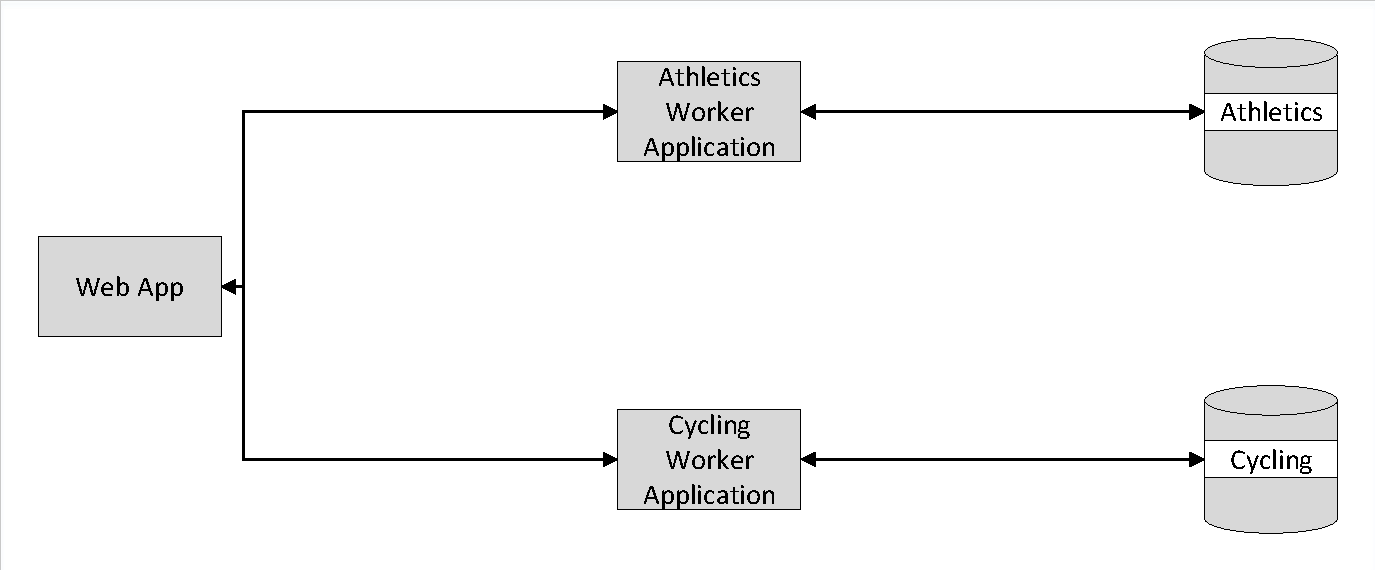
\includegraphics[trim = 5 5 5 5, clip, width=\textwidth]{img/simplemicro}
\end{figure}

%
% ---- Operational microservices
%
\subsection{Operational microservices}

A more 'natural' microservices archtecture partitions the system by operation (Book, Search, Return) with a separate database for each.  The databases maintain eventual consistency via an event streaming application e.g. using Kafka.
\begin{enumerate}
\item Book is an event producer and consumer (produces when a ticket is booked, consumes returned tickets).
\item Search is an event consumer (consumes the state of tickets that are booked and returned).
\item Return is an event producer (produces returned tickets).
\end{enumerate}

\begin{figure}
	\caption{Operational microservices architecture}
	\centering
	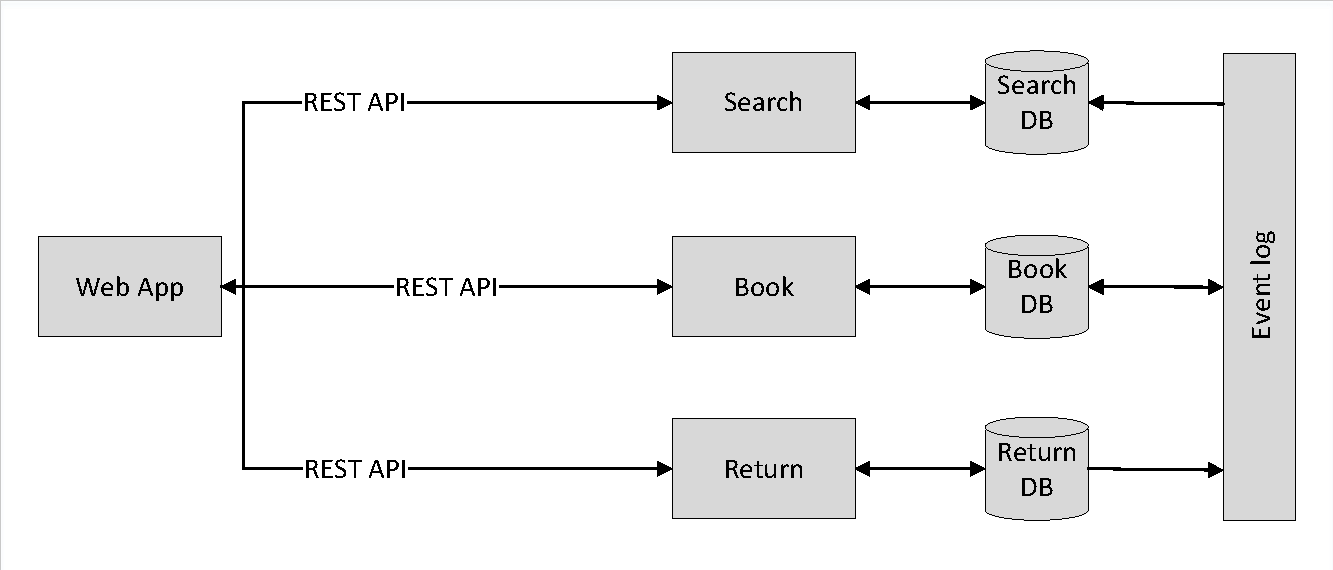
\includegraphics[trim = 5 5 5 5, clip, width=\textwidth]{img/operationmicro}
\end{figure}

%
% ---- Shared queue middleware
%
\subsection{Shared queue middleware}

Requests via a shared queue to worker applications going to a distributed database with two nodes, Athletics and Cycling.

\begin{figure}
	\caption{Shared queue middleware architecture}
	\centering
	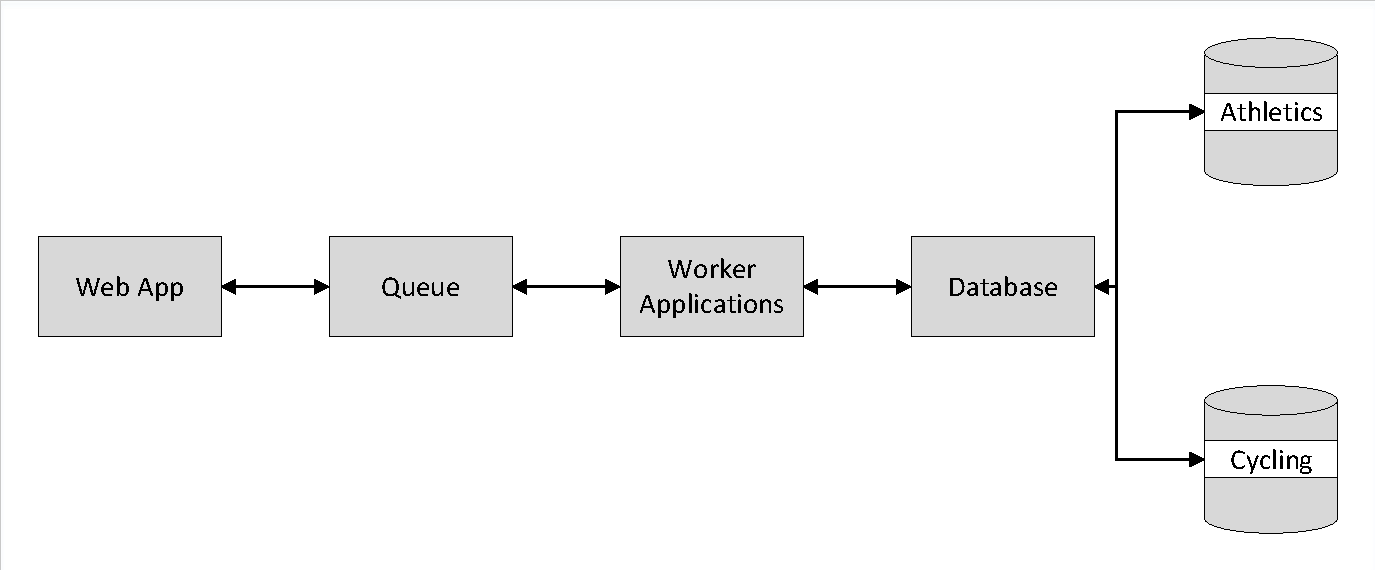
\includegraphics[trim = 5 5 5 5, clip, width=\textwidth]{img/sharedqueue}
\end{figure}

%
% ---- Distributed database with replication
%
\subsection{Distributed database with replication}

Requests via a shared queue to worker applications going to a distributed database with three nodes, Athletics, Cycling and Diving, where each partition is replicated on another node.

\begin{figure}
	\caption{Distributed database with replication architecture}
	\centering
	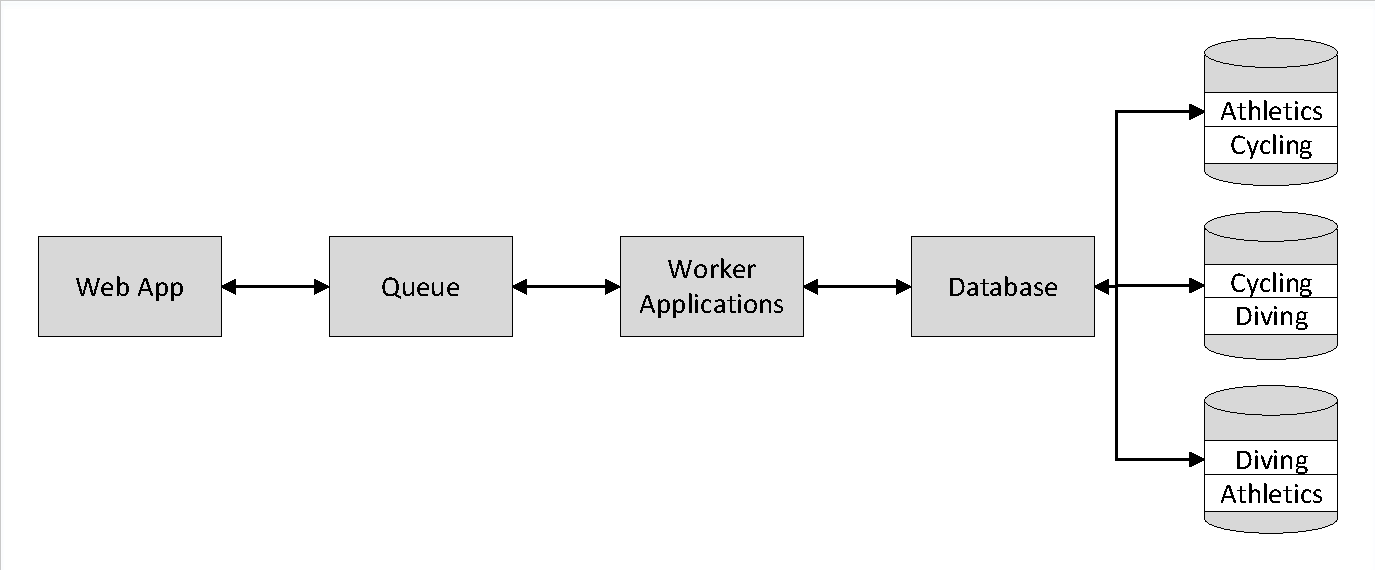
\includegraphics[trim = 5 5 5 5, clip, width=\textwidth]{img/sharedqueue_withrep}
\end{figure}